\chapter{Aufgabe 4: Quicksort}
\section{Performanzvergleich}
Die Laufzeiten der sequentiellen und mit OpenMP parallelisierten Quicksortalgorithmen ergeben sich wie folgt:\\ \\

\begin{center}
\begin{tabular}{l|c|r}
Anzahl Elemente & Laufzeit parallel & Laufzeit sequentiell \\
\hline
$10^5$ & 19 ms & 10 ms \\
$10^6$ & 78 ms & 80 ms \\
$10^7$ & 242 ms & 970 ms \\
\end{tabular}
\end{center}

\begin{figure}[H]
    \centering
    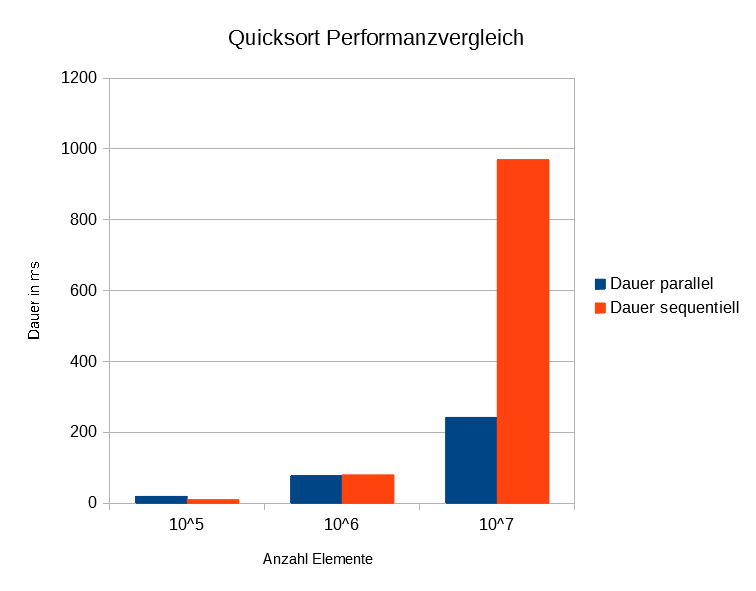
\includegraphics[width = \textwidth]{img/qs_performance_comparison.png}
    \caption{Performanzvergleich für Quicksort}
    \label{qs_perf_comp}
\end{figure}

\section{Parallelisierung von rand()}
Um parallelisiert zu werden, müsste rand() ein reproduzierbares Verhalten aufweisen. Dies ist nicht gegeben, da in jedem Thread, bei jedem Aufruf von rand() Parameter verändert werden, die die Generierung der Pseudozufallszahlen beeinflussen. Die benötigte Eigenschaft einer Funktion, um sicher in mehreren Threads ausgeführt werden zu können, ist Eintrittsinvarianz. Dies bedeutet, dass die Funktion unterbrochen werden kann und nach Wiedereintritt immer noch das gleiche erwartete Ergebnis liefert wie bei einem unterbrechungsfreien Durchlauf.
